%!TEX root = ./intern_report.tex

\subsection{Company Overview}

\paragraph{}
Wave Computing is a USA Silicon Valley based company that specializes in dataflow technology~\cite{waveintro}, an alternative to the tensorflow~\cite{tflow} technology used by tech giants such as {Nvidia} and {Google} to accelerate {AI} and neural net training. Although the company is relatively new to the game, they have had a number of notable achievements, which are explained below in detail. They outsource their design contracts to teams around the globe and one of these contracts was undertaken by Paraqum Technologies. This particular team works with the Software development kit ({SDK}) and the applications of the Wave dataflow platform.
\begin{figure}[h]
    \centering
    
\includegraphics[trim=0cm 0cm 0cm 0cm, clip=true,scale=1]{figures/wave_logo.png}
    \caption{Wave Computing logo\label{Fig:Wave}}\vspace{-4mm}
    \end{figure}


\paragraph{}
Paraqum Technologies is one of the very first truly Sri Lankan Electronics industry companies in the country. It undertakes Electronic design contracts from big companies from around the world such as Osprey video and of course, Wave Computing. They also have their own network product line. The company had one of their teams working on a design project of Wave Computing which split up in November 2018 to form the Sri Lankan branch of Wave Computing (pvt) Ltd. 
\begin{figure}[h]
    \centering
    
\includegraphics[trim=0cm 0cm 0cm 0cm, clip=true,scale=1]{figures/pqm_logo.png}
    \caption{Paraqum Technologies logo\label{Fig:Paraqum}}\vspace{-4mm}
    \end{figure}

\paragraph{}
My work was focused on the SDK layer of the Wave dataflow platform. This describes a large toolchain of software utilities that are the primary way that an advanced user would interact with the system. This team is also one of the busiest teams of the whole organization because of the sheer complexity of the SDK. In the context of the Sri Lankan staff, the SDK team is the heart of the whole project.


\subsection{Company History - Wave Computing}

\paragraph{}
Wave computing is primarily a project-turned-to-startup by Dr. Derek Meyer, who is also the current CEO. The idea is to design a processor to process the huge amount of data required for complex operations such as large matrix multiplication applications in parallel. He realized his idea in to a semiconductor manufacturing company, wave semiconductor, which has become a legacy as some urls of the company still reads 'wavesemi'. As the prospect of Artificial intelligence became popular, the company understood that their time and effort is best invested in that field and hence, wave semiconductor reformed into Wave Computing AI.

\paragraph{}
To meet the demand for Artificial intelligence applications, wave computing has planned a series of devices which can fit the requirement of the users whether it is a large datacenter or a small scale business or mobile/{IoT} devices.
\begin{figure}[h]
    \centering
    
\includegraphics[trim=0cm 0cm 0cm 0cm, clip=true,scale=0.5]{figures/wave_server.png}
    \caption{Wave Datacenter Server Unit\label{Fig:waveserver}}\vspace{-4mm}
    \end{figure}

\begin{figure}[h]
    \centering
    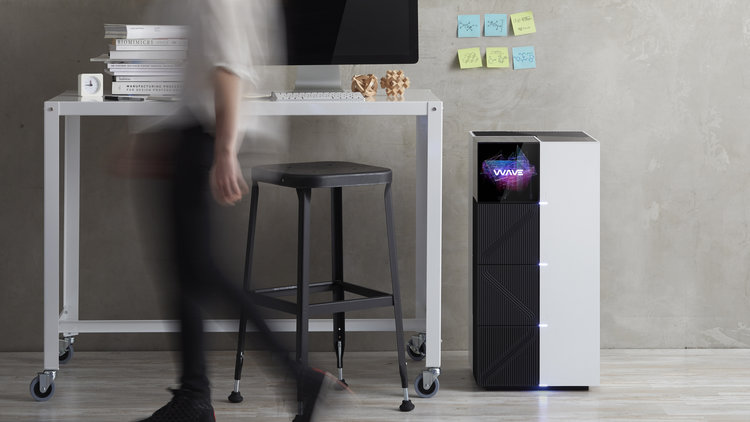
\includegraphics[trim=0cm 0cm 0cm 0cm, clip=true,scale=1]{figures/wave_lab.jpg}
    \caption{Wave Consumer Unit\label{Fig:wavelab}}\vspace{-4mm}
    \end{figure}

\subsection*{MIPS Acquisition}
\paragraph{}
MIPS is one of the old time giants of the silicon design game. To facilitate their ideology of integrating dataflow technology to small devices, Wave Computing recently acquired MIPS~\cite{mipsaq} for their silicon design expertise. With this step, Wave computing hopes to realize their idea of "Bringing datacenter to the edge" by installing datacenter level high performance hardware in small(edge) devices.

\subsection{Company History - Paraqum Technologies}
\paragraph{}
Started in 2013 as a continued final year project of four students from the 2008 batch of University of Moratuwa Department of Electronic and Telecommunication Engineering, Paraqum Technologies was first located inside the university itself. The CEO also being a lecturer in the University, this was the result of the attempt to promote technical entrepreneurs to rise up from the university level.

\paragraph{}
Paraqum Technologies quickly developed into a full sized technology startup and by 2018, the staff had grown to around 40 and every year they took around 10-12 interns under their wings to properly expose them to the electronic industry. Now they have design contracts from renowned industrial leaders and their own networking product line which is also very famous for their unique capabilities.

\begin{figure}[h]
    \centering
    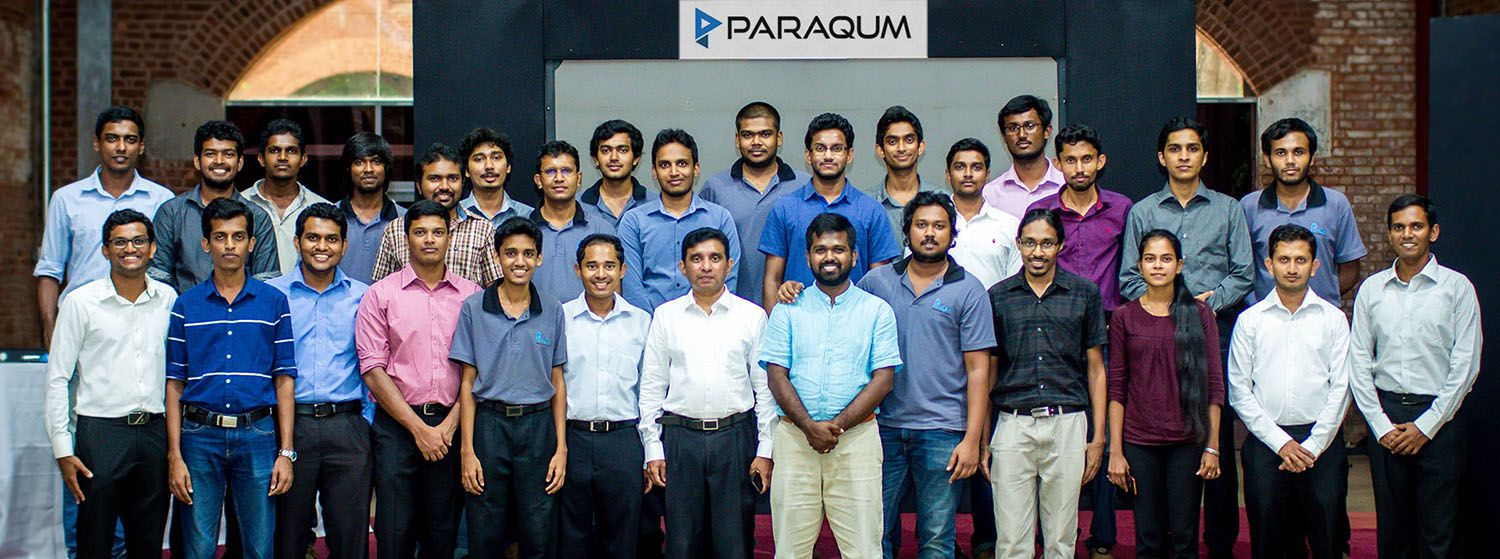
\includegraphics[trim=0cm 0cm 0cm 0cm, clip=true,scale=0.25]{figures/paraqum_team.jpg}
    \caption{Paraqum Technologies Staff (including Wave team members)~\cite{pqmintro} \label{Fig:pqmteam}}\vspace{-4mm}
    \end{figure}

\subsection{Wave-Paraqum partnership, separation and its effect on interns}

\paragraph{}
As described above, Paraqum Technologies had a design contract from wave computing for their toolchain and application needs. This contract had been in place for almost two years and has proved to be one of the most productive teams wave computing has ever employed. They have helped in designing the hardware part of the dataflow processing chips and by the time we started our internships, they were working on RTL level software projects.

\paragraph{}
However, Wave computing had decided it would be better to acquire the Sri Lankan team for themselves. So, in november 2018, the Wave Computing team was separated from Paraqum Technologies and established as the Sri Lankan branch of Wave Computing (pvt) ltd. with no connection to Paraqum Technologies whatsoever. Before Separation, Wave computing team worked in the Paraqum Technologies office in Kohuwala but after that they moved to a new office in Bambalapitiya.

\begin{figure}[h]
    \centering
    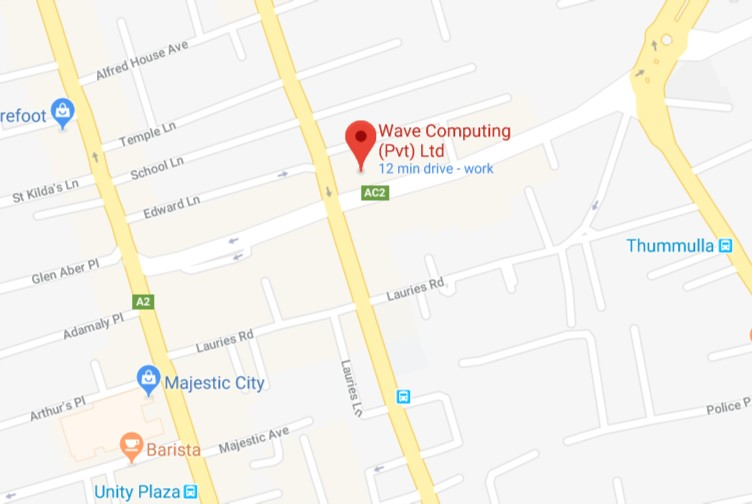
\includegraphics[trim=0cm 0cm 0cm 0cm, clip=true,scale=0.25]{figures/wave_location.jpg}
    \caption{Wave Computing Office location \label{Fig:pqmteam}}\vspace{-4mm}
    \end{figure}

\paragraph{}
As the organizations separated, interns of the wave team also moved to work in the new office premises and work was carried out as normal. But the internship contracts were not changed and technically, we were interns of Paraqum Technologies for the whole 24 weeks but worked under the supervision of Wave Computing staff. Therefore this report will be more focused on Wave Computing.

\subsection{Organization Structure and Hierarchy}

\paragraph{}
Wave computing team was another division in Paraqum Technologies until the separation but after that they became a fully independent entity. The dotted line in the following diagram represents the administration link that existed before the separation. Now Wave computing Sri Lanka operates directly under the administration of their head office in Campbell, California. 

\begin{figure}[h]
    \centering
    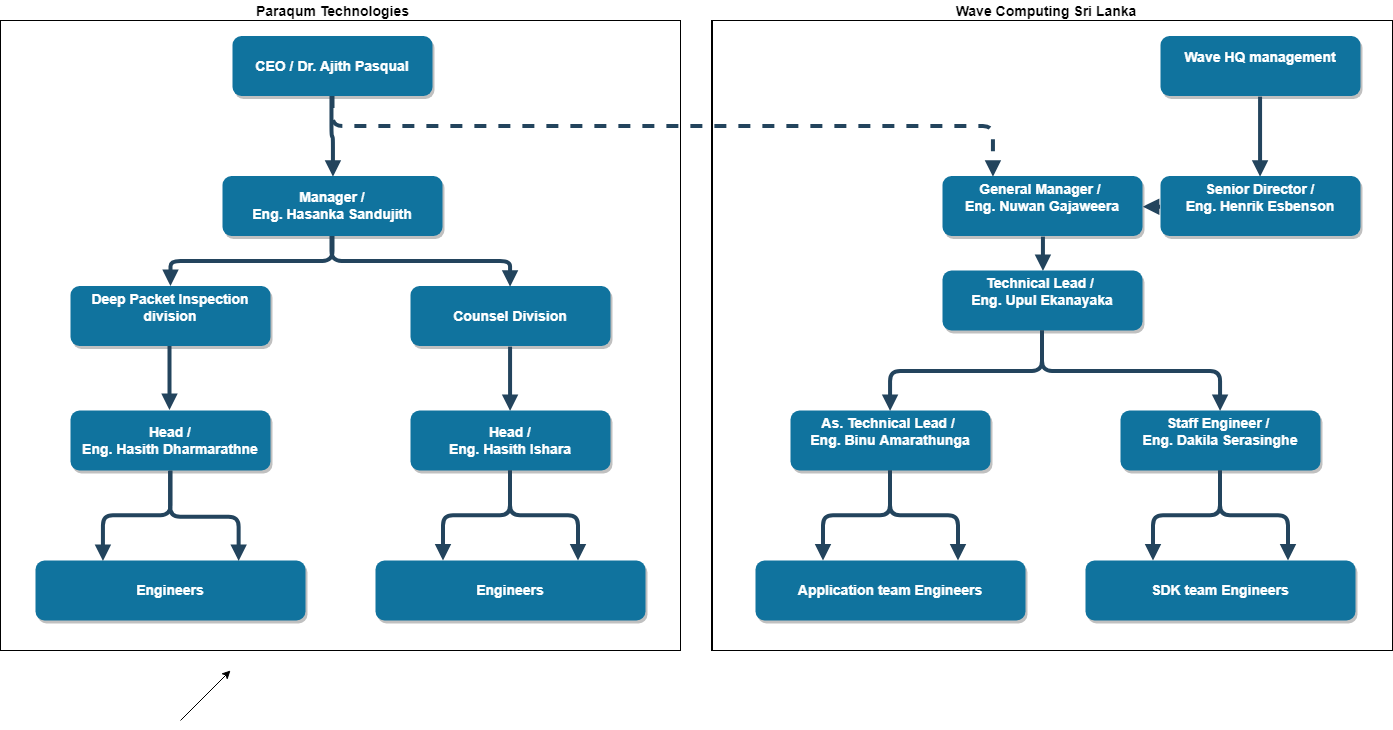
\includegraphics[trim=0cm 0cm 0cm 0cm, clip=true,scale=0.25]{figures/admin_struct.png}
    \caption{Wave/Paraqum administration structure \label{Fig:adminstruct}}\vspace{-4mm}
    \end{figure}

\subsection{Areas of Interest}

\begin{figure}[h]
    \centering
    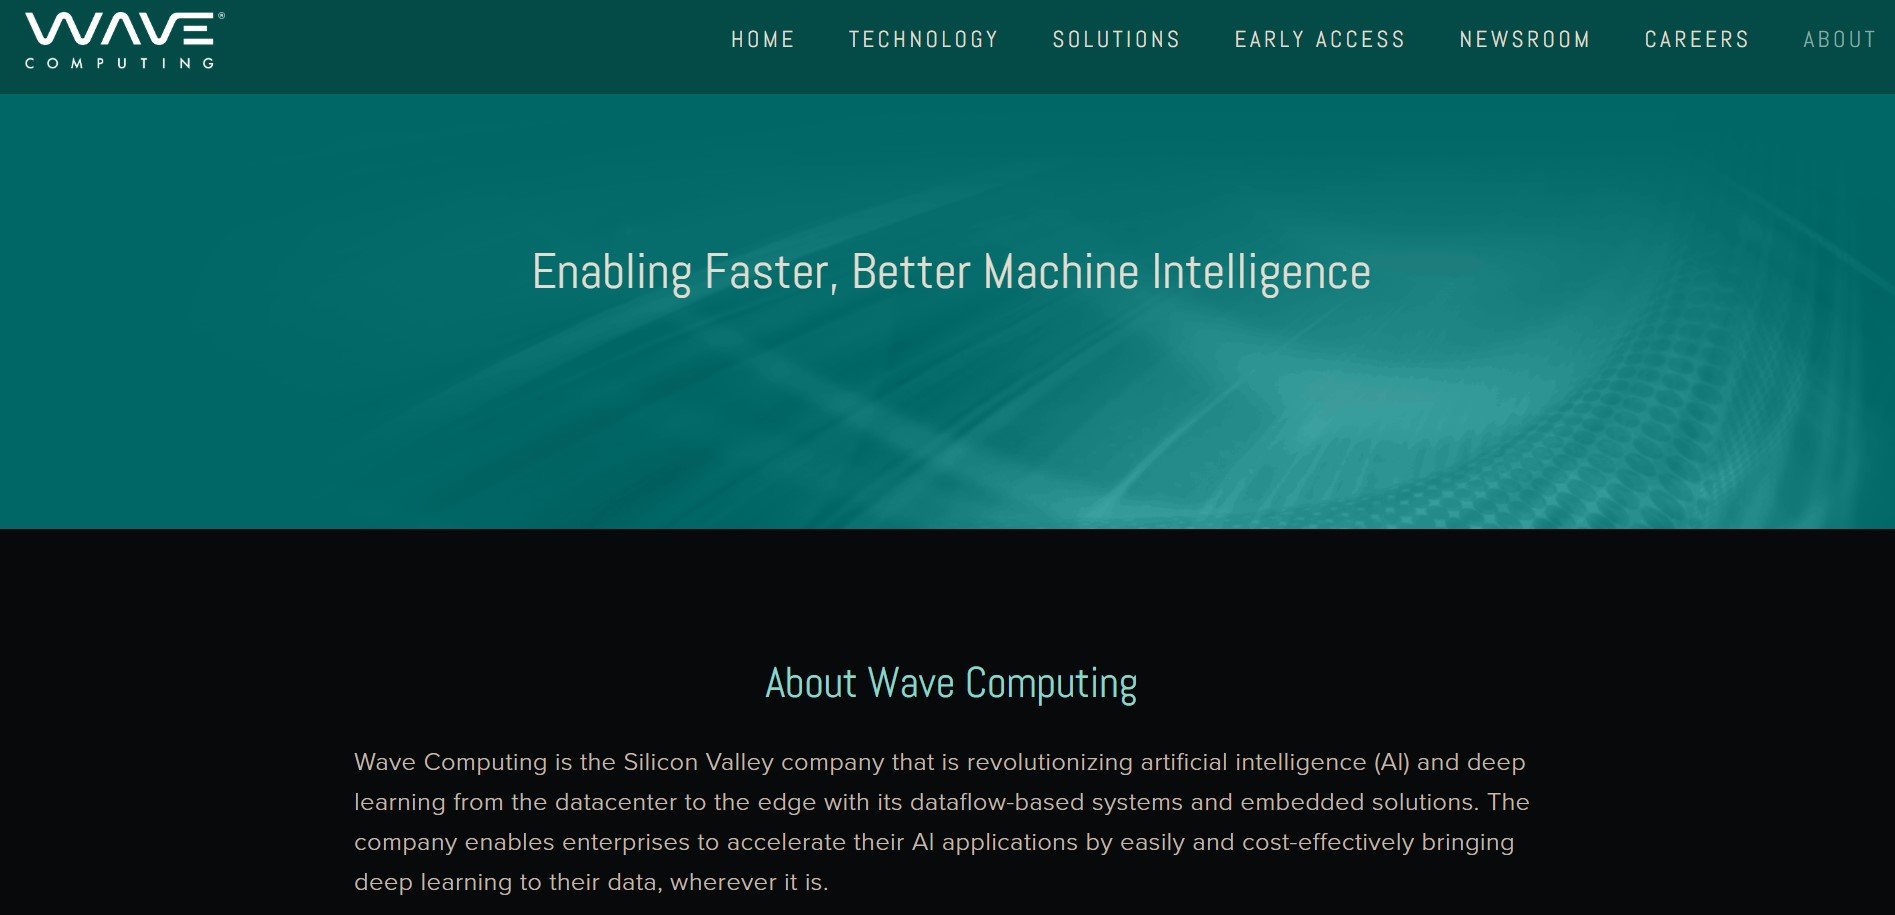
\includegraphics[trim=0cm 0cm 0cm 0cm, clip=true,scale=0.25]{figures/wave_site.jpg}
    \caption{Wave computing Homepage with their target of better AI\label{Fig:wavesite}}\vspace{-4mm}
    \end{figure}

\paragraph{}
The main focus of Wave computing is to Introduce new processing system for heavy computational operations with their proprietary dataflow processing technology. When the system is built and released, it can be used for:

\subsubsection*{Artificial Intelligence}
\paragraph{}
The main use of the dataflow processing units (DPU) is intended to be Artificial Intelligence systems. Current hardware in our devices are not suited for the massive amount of data that need to be processed in parallel. The DPU has been optimized for this particular task to perform it at high speed. It is speculated that once wave DPU systems become available in market, it will spark a revolution in the AI industry.

\subsubsection*{Edge devices}
\paragraph{}
Edge devices are small devices such as mobile phones and IoT sensors. Wave computing already has plans in motion to develop high performance, small size hardware to be installed in these edge devices. This will allow us to have very powerful yet small devices for our day to day usage.

\subsubsection*{Image processing}
\paragraph{}
Image processing and AI are similar in many ways. The parallel data handling capacity of DPU systems makes it an ideal candidate for image processing applications such as self driving or biometric authentication.


\subsection{Current Situation}
\paragraph{}
The initial release of Wave hardware to the general public is scheduled for 2020 and the company is doing well on the roadmap to meet this target. The hardware design is nearly perfect and the software is halfway through. It can be expected that the company will meet the target soon enough and they are expanding rapidly now, with the new office in Sri Lanka hiring more and more people. 


\subsection{Impacts on Sri Lankan Industry}
\paragraph{}
Having recently completed a very successful series E funding round~\cite{fund}, Wave Computing has a fairly large capital at its disposal and are ready to invest well in the Sri Lanka division. This huge amount of money will directly enter Sri Lankan economy in US dollars, aiding the stabilization of economy. They also offer employment to talented local engineers in bigger and bigger numbers every year. Finally, when the Wave product line enters market and becomes a key element in the AI game, Sri Lankans will have an important role to play in it, carrying us forward in the technical development sector.

\newpage
\subsection{SWOT Analysis}

\subsubsection*{Strengths}

\begin{itemize}
    \item Wave already has MIPS under them, giving them a considerable head start on the silicon game. They got a team of experienced engineers with this acquisition.
    \item They have teams around the world with different perspectives, allowing creative solutions to problems.
    \item The company is very well funded, giving them plenty of runway.
    \item The startup culture is well maintained in the workplaces, making it appealing to employees.
\end{itemize}


\subsubsection*{Weaknesses}
\begin{itemize}
    \item Without any kind of product on the market yet, the company solely runs on VC funding
    \item Global teams sometimes cause delays in communications.
\end{itemize}


\subsubsection*{Opportunities}
\begin{itemize}
    \item AI field is expanding day by day, meaning the potential market for the company widens continuously.
    \item Another funding round can result in more and more funds due to the promising nature of the project.
    \item Reputation of the company is luring in more talent as it expands.
    \item Since the hardware is not restricted only to AI applications, there can be more potential uses to the devices.
\end{itemize}

\subsubsection*{Threats}
\begin{itemize}
    \item There may be rival companies with better solutions to the AI processing problem than the DPU technology.
    \item Some of the global teams are from politically and economically unstable countries and they might be lost to national crisis.
    \item DPU is not fully built yet. It may not give the expected outcomes and performance in real world.
\end{itemize}

\subsection{Suggestions to Improve the Company}
\begin{itemize}
    \item Some sort of outbound activities can be organized to allow the team to bond even better.
    \item Interns could be provided with some more training sessions.
\end{itemize}